\documentclass[parskip=true, 10pt]{scrartcl}
\usepackage[utf8]{inputenc}

\usepackage[top=1.0in, bottom=1.4in]{geometry}
\usepackage{hyperref}
\usepackage{tabularx}
\usepackage{url}
\usepackage{float}
\usepackage{graphicx}
\usepackage{enumerate}
\usepackage{booktabs}
\usepackage{color}
\usepackage{enumitem}
\usepackage{amsmath}

\title{\vspace{-1cm}IoT Linear Integrate \& Fire\\\vspace{0.4cm}{Final Report}\vspace{0.5cm}}

\author{
  \textbf{\textsf{Simon Kaufmann}} \\
  \texttt{sikaufma@ucsd.edu}
  \and
 \textbf{\textsf{Owen Jow}} \\
  \texttt{owen@eng.ucsd.edu}
}
\date{June 2020}

\begin{document}

\maketitle

\tableofcontents

\section{Abstract}

% FIXME Insert percentage and network parameters etc.
% No more than 120 words
Due to the growing need for communication services to share a limited frequency spectrum, the ability to classify signals by modulation has risen in importance. At the same time, the desirability of small, low-cost communication devices means that efficiency of the solution is almost as important as efficacy. With this in mind, our method leverages spiking neural networks (an emerging event-based variant of traditional neural networks) to perform modulation classification more efficiently than previous approaches. We train a model using deep continuous local learning, quantize the parameters, and validate our approach on the RadioML dataset, a publicly available collection of I/Q radio signals. Using this method, we achieve a peak accuracy of 56\% with 955K network parameters. We also propose a quantized model with 8-bit precision for static parameters and 24-bit precision for runtime parameters, where the quantization accounts for a drop in accuracy of around 1.5\%. These results represent a first step toward an efficient, event-driven solution for signal classification.

% Improvements:
% Cons:
% Could not find the detail of background. (‘adaptive cognitive radios’)
% Could have expanded more on approach (‘what was done previously’, ‘order of actions’)
% Vague results (x,y,z is unrelated ) -- No result (may be too early)


\section{Introduction}

% Higher level overview of the research area
% Summarize in bullet points contributions of the research area

% Contributions
% - Examine suitability of SNN trained using DCLL for modulation classificaition (on RadioML dataset)
% - Adapt DCLL library to use Brevitas features for quantization-aware training
% - Explore impact of quantization on SNNs trained using DCLL
% - Propose architecture of SNN for RadioML
% - Propose architecture of quantized SNN

Radio communication plays an important role in modern-day life and shapes the way people are able to communicate with each other through mobile devices. A growing number of communication services (like the 5G mobile phone network) need to share a very limited frequency spectrum. The ability to share the same frequency range for different services is thus very useful, but requires being able to classify and recognise received radio signals by the service they belong to. To achieve this, our project uses spiking neural networks in conjunction with the RadioML dataset for training and evaluation.

The RadioML dataset \cite{radioml-dataset} is a publicly available dataset of radio signals of 24 different modulation classes and 26 different signal-to-noise ratios. Different deep learning architectures have previously been used to create models for classifying RadioML data \cite{previouswork} and have achieved a classification accuracy of up to 95\% on data samples with high signal-to-noise ratios (close to 30 dB).

Spiking neural networks are event-based neural networks based on biological neurons. They receive input in form of discrete events (spikes) which cause the internal neuron state to change (membrane potential). Once the internal state of individual neurons reaches a certain threshold, the neurons themselves cause further events (spikes) to be forwarded to connected neurons.

While SNNs are considered relatively \lqq hardware-friendly\rqq\ and allow for energy-efficient implementation on low-cost devices, they generally achieve lower accuracy than regular neural networks (convolutional networks, etc.) as per \cite{snn-survey}. Thus, when considering SNNs, and especially when first seeing their associated classification accuracies, it is important to keep in mind those aforementioned advantages -- that they can help produce lightweight, low-power and low-cost applications.

The goal for this project is to implement and optimize a spiking neural network for modulation classification on the RadioML dataset and to quantize the SNN in order to provide an efficient version that can be implemented on an FPGA in the future.

For the quantization, we use a sofware package called Brevitas which supports quantization-aware training of neural networks. We adapted Brevitas to work together with the DCLL library for creating SNNs.

An overview of the used software parts is shown below:

\begin{figure}[H]
    \centering
    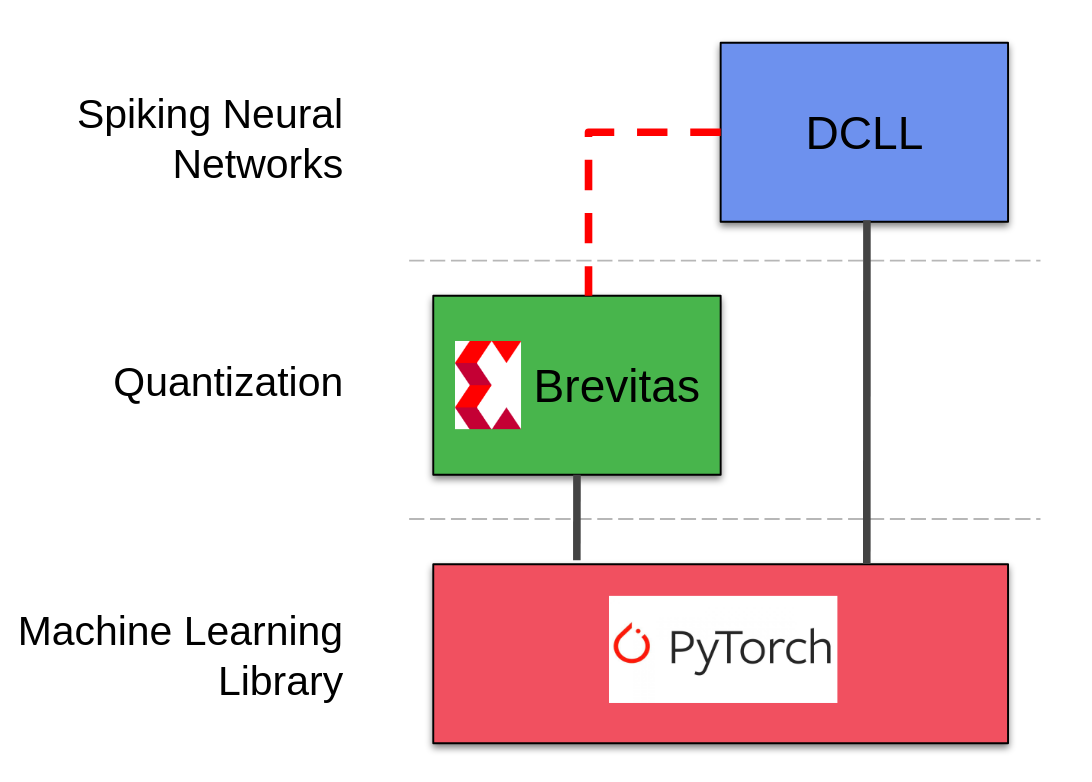
\includegraphics[width=0.5\textwidth]{brevitas-graphic.png}
    \caption{Overview of software parts for the project.}
\end{figure}

The contributions of our work are as follows:
\begin{itemize}
    \item We have made, to the best of our knowledge, the first attempt at applying spiking neural networks to the task of modulation classification for radio signals.
    \item We have also optimized different parts of our model (state and weights) using quantization methods and adapted the DCLL library for compatibility with Brevitas.
    \item Since our accuracy is still slightly below that of the worst-performing traditional networks from previous papers, the main advantage of our method is the fact that it is event-based and can be run more efficiently on specialized neuromorphic hardware.
\end{itemize}

\section{Technical Material}

% Bulk of the report

\subsection{Spiking Neural Networks and DCLL}

A spiking neural network (SNN) is a variant of a neural network that utilizes spike-based communication over continuous time in accordance with actual biological neuron models. In this way, it can be seen as a special case of a binary, recurrent neural network. However, while SNNs use a more complex and powerful neuron model and are naturally equipped to capture temporal dynamics, they suffer from very underdeveloped training methods in relation to traditional neural networks. In particular, they are difficult to train because spikes over time are non-differentiable, and the biological neuron model decrees that computation should remain local to each neuron, meaning we cannot simply backpropagate through time (backpropagation through time tends to be prohibitively expensive with regard to memory anyway).

Fortunately, one recent paper (\cite{DBLP:journals/corr/abs-1811-10766}) provides a convenient way to implement and train spiking neural networks using local layer-wise gradients which are only backpropagated within the same layer and time step. Their method is called ``deep continous local learning," or DCLL for short. In DCLL, each layer is itself trained to solve the classification task (although the spiking output is still passed to the next layer), in that a frozen fully-connected reduction of the layer output is optimized to predict the correct class probabilities. This ensures that each layer learns useful features for solving the relevant task.

In the DCLL formulation of a spiking neural network, each neuron maintains extra state variables that are propagated forward in time. Because this information is sufficient for computing gradients at the next time step, DCLL allows for memory-efficient training.

As per \cite{DBLP:journals/corr/abs-1811-10766} and the associated public codebase, the dynamics of the spiking neural network under DCLL can be described by the following equations:
\begin{align*}
    Q^l(t + \Delta t) &= \beta Q^l(t) + \frac{1}{1 - \beta}S^{l-1}(t) \\
    P^l(t + \Delta t) &= \alpha P^l(t) + \frac{1}{1 - \alpha}Q^l(t) \\
    R^l(t + \Delta t) &= \gamma R^l(t) - (1 - \gamma) S^l(t) \\
    U^l(t + \Delta t) &= \texttt{conv}(P^l(t + \Delta t)) + R^l(t + \Delta t) \\
    S^l(t + \Delta t) &= 1 \text{ if } U^l(t + \Delta t) \geq 0 \text{ else } 0
\end{align*}
where $l$ denotes the layer, $t$ denotes the time step, $S^l$ is the output spike image for layer $l$, and $P, Q, R, U$ are synaptic, refractory, and membrane-related state variables. $\Delta t$ denotes the length of the time step. Note that the values of $P^l$, $Q^l$, $R^l$, and $S^l$ are each passed to the next time step in the same layer, so these variables encapsulate the ``state" of a neuron in a layer. One important point is that although these state variables are passed to the next time step, their gradients neither need nor will be allowed to propagate backward through time (resulting in a critical savings in memory, as we do not need to keep track of the entire computation graph for multiple time steps).

\begin{figure}[h]
    \centering
    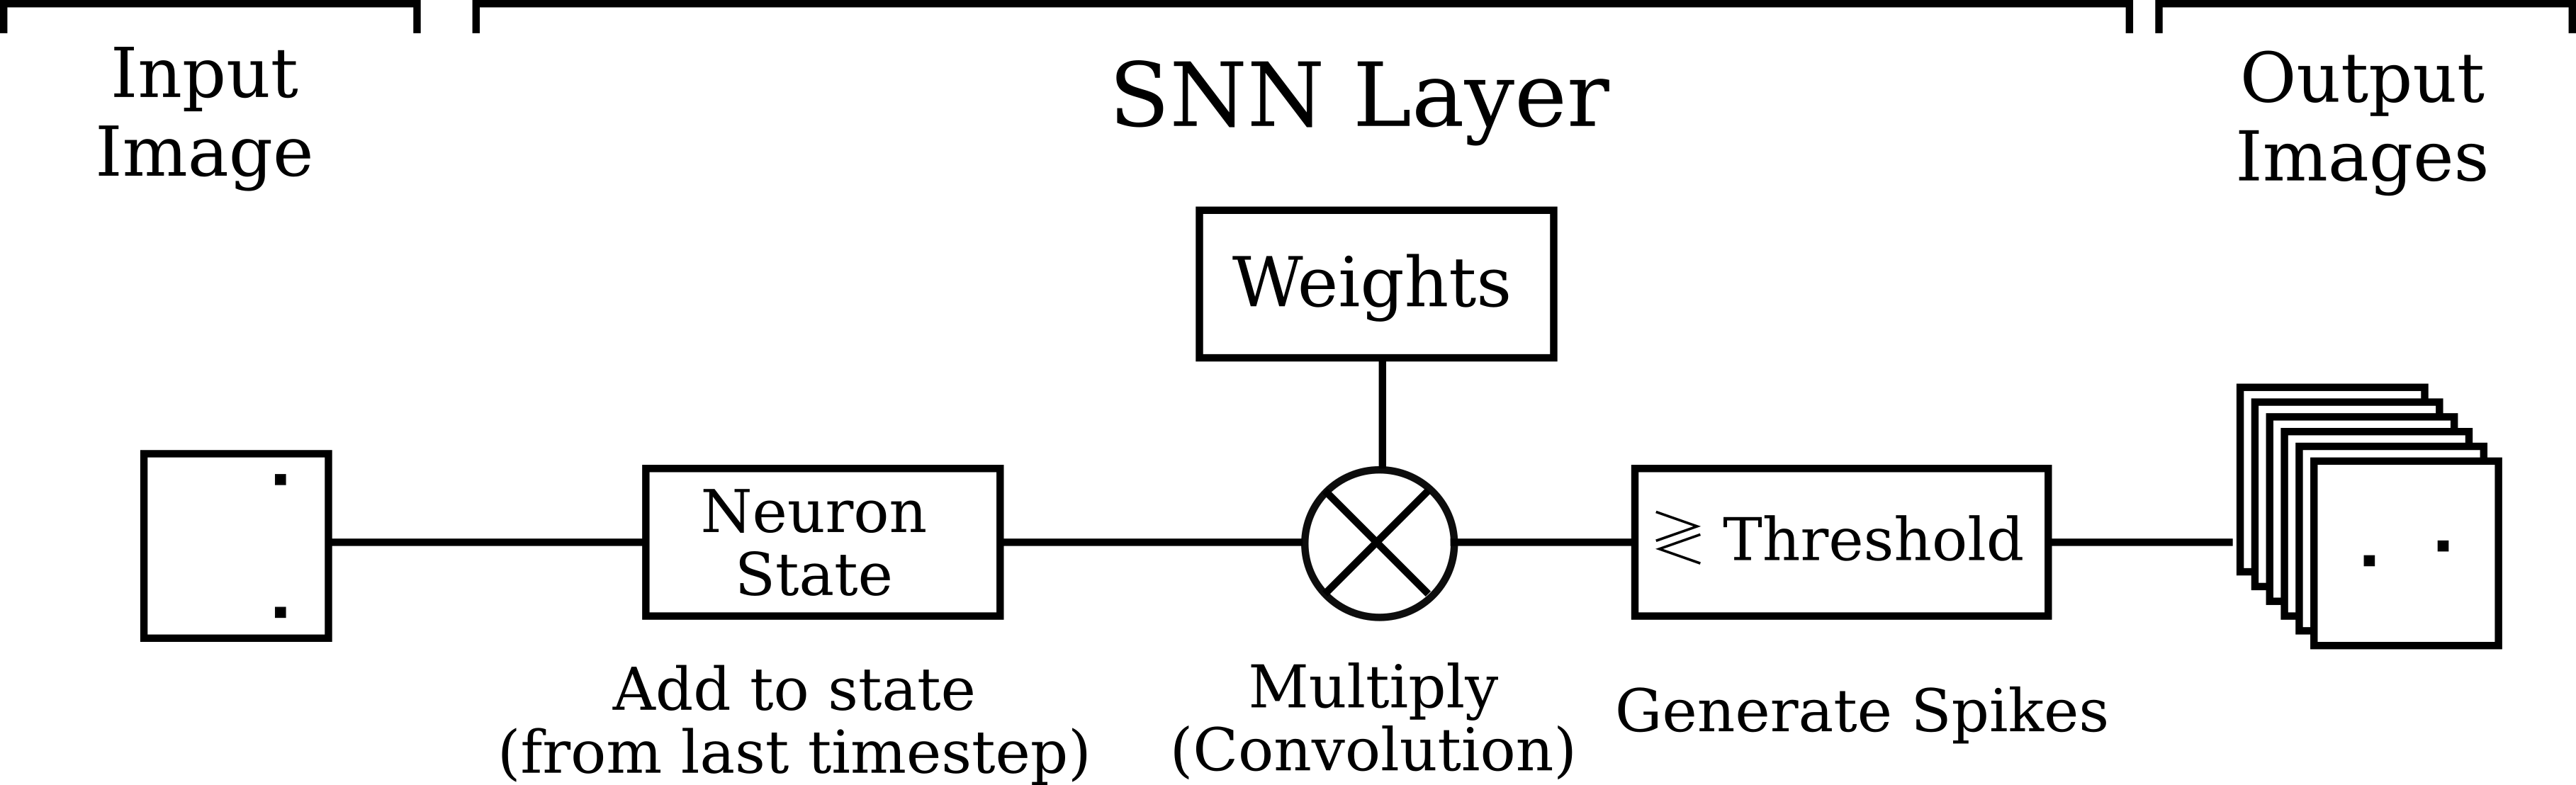
\includegraphics[width=0.8\textwidth]{spiking-layers.png}
    \caption{Simplified view of a convolutional DCLL spiking layer.}
    \label{fig:snn_neuron}
\end{figure}

\subsection{RadioML}

We train and evaluate our method on radio signals from the RadioML dataset. This dataset consists of 2.5 million radio signals formatted as I/Q samples over 1024 time steps each. Each signal is labeled with its modulation class (one of 24) and SNR (one of 26, with the minimum SNR being -20 dB and the maximum SNR being +30 dB). Following \cite{previouswork}, we only train on SNRs from +6 dB to +30 dB.

Although previous deep learning approaches have typically fed the entire 1024-length signal to the network at once (as a 1D signal with two channels), we would like to provide our spiking neural network with a spiking input for each time step. Therefore, we transform each I/Q sample (a tuple of two numbers representing the real and imaginary components of the signal at a time step) into an image by plotting the I/Q sample on the I/Q plane and discretizing the plane over the range $[-1, 1]$ in each dimension. This way, one could imagine each data point in the signal arriving one after another (as events) to the SNN, which would provide class predictions in real time.

\begin{figure}[H]
    \centering
    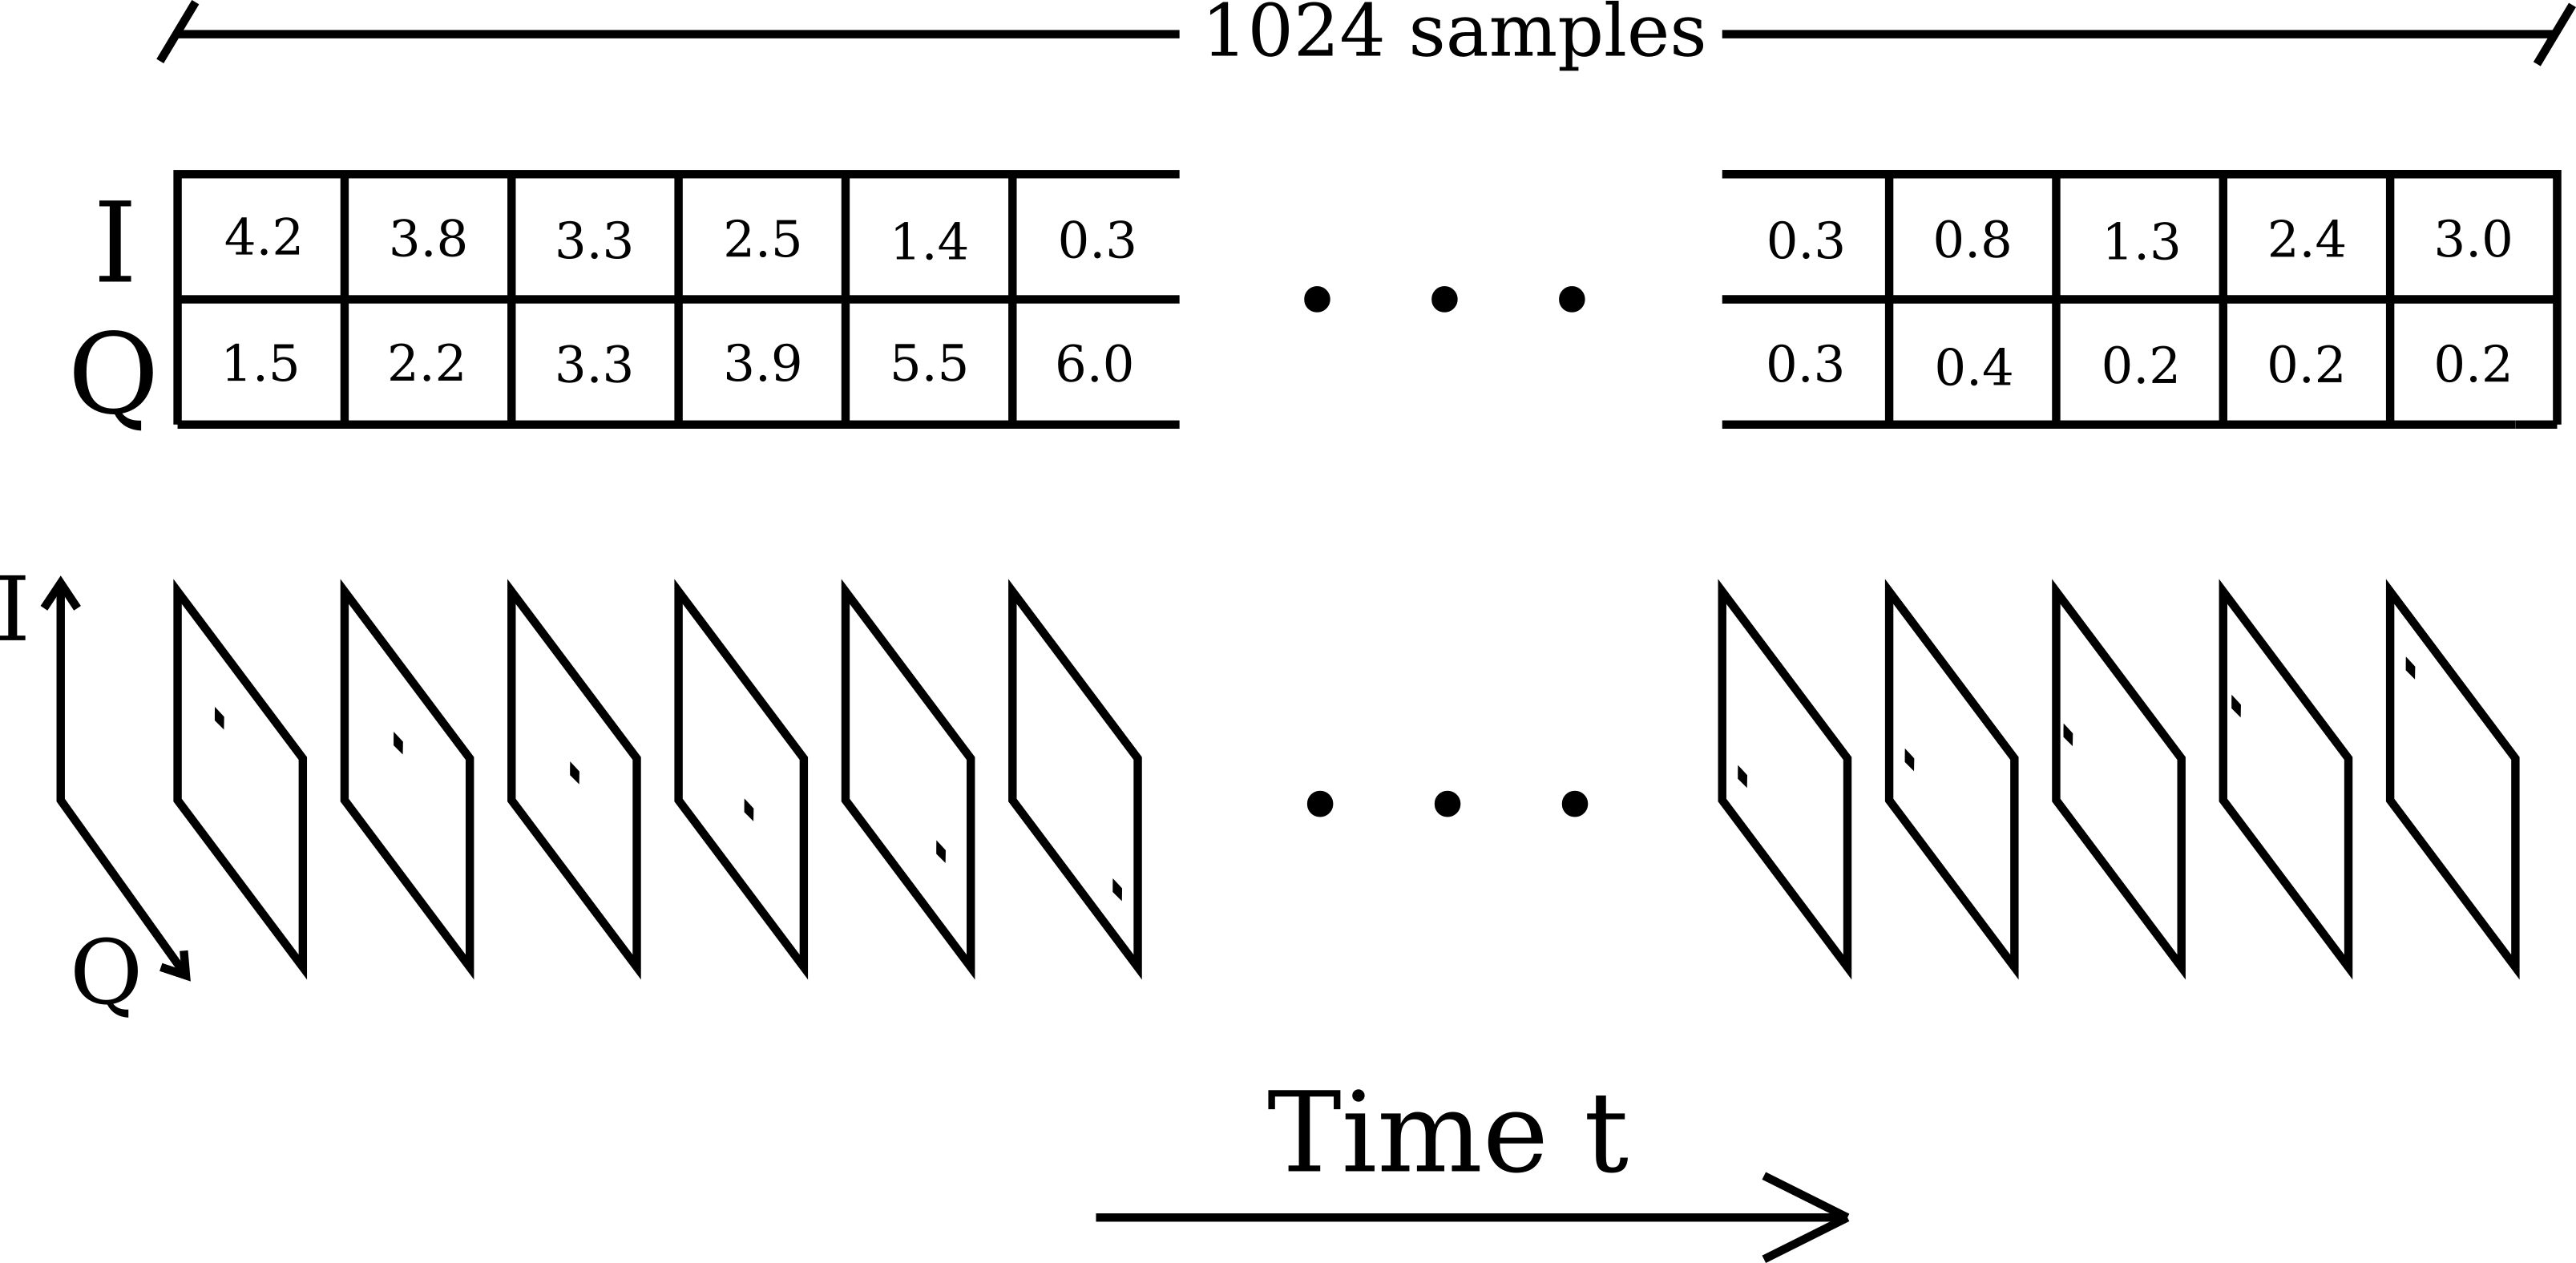
\includegraphics[width=0.8\textwidth]{radioml.png}
    \caption{A visualization of image discretizations for I/Q samples.}
    \label{fig:radioml_iq_images}
\end{figure}

\subsection{Brevitas}
\label{sec:brevitas}

Brevitas is a machine learning library based on PyTorch for quantization-aware training. While conservative quantization (keeping the bit-width relatively high) may be possible retrospectively after the training process without too much loss of accuracy, quantization for very low bit-width (e.g. 2- and 4-bit) can often achieve better results
if the  model is trained using the quantized forward pass. Brevitas assists with adjusting PyTorch models and optimizing them for use in scenarios which require quantization.

For this purpose, Brevitas defines various classes that can be used similarly to the conventional PyTorch classes, e.g. \texttt{QuantConv2D} and \texttt{QuantLinear}. Each of these classes support detailed settings to specify the nature of the quantization, e.g. the minimum and maximum bit-width, the method of converting numbers to integers and scaling factor, and whether or not rescaling will be applied.

Brevitas defines a \texttt{QuantTensor} which is used as the quantized version of a regular \texttt{Tensor} in PyTorch. It is implemented as a named tuple containing three values: the actual tensor, the scale factor, and the bit width. The actual tensor corresponds to the regular PyTorch tensor object. The values in this tensor are still floating point numbers, but they will only be set to values that correspond to the correct quantized grid---essentially this tensor contains the integer values multiplied by the scale factor. 
The second tensor in the tuple contains only one element which is the scale factor that was applied to the integer values, and the third tensor contains the bit width that was used for the \texttt{QuantTensor} -- for example if
the bit width is 2, there are only four values allowed in total in the first tensor. The scale factor determines which values are allowed.

\subsection{Tuning of SNN for RadioML network}

We tried a lot of different hyperparameter settings in order to train the SNN on RadioML data. Dimensions that we varied included, among other things: the resolution of the discretized I/Q images, the ranges of the dicsretized I/Q images, the regularization weights, the network architecture (number of filters in each layer, severity of pooling, kernel sizes, different padding sizes and types, number of convolutional layers, number of dense layers, spiking versus non-spiking dense layers), the constants for the spiking neuron dynamics, the activation functions, dropout probabilities, additional dropout layers, different sampling weights for different classes and SNRs, different SNRs used for training, different subsamplings of the data, continuing the training of pre-trained networks with different settings, different data preprocessing (e.g. wider spikes, ``gamma correction" for different and nonlinear discretizations of the [-1, 1] range in order to put more pixels in the parts of the range where there were more samples, difference images -- including an extra event for spikes being removed from the previous time step), increased burn-in times (where training updates don't happen), different fixed signal durations during training, randomized burn-in and start times and signal durations during training, random noise injection, and learning rates (including different learning rates for each layer). 

\subsection{Proposed Architecture and Results}

Ultimately, our best-performing architecture ended up containing three convolutional layers with 32 learned $7 \times 7$ kernels in each layer (and length-3 zero padding on each side), followed by a fully-connected layer and a softmax activation to reduce the intermediate results to class probabilities. Each layer was, of course, a spiking DCLL layer wrapped around these base layer types.

\begin{figure}[H]
    \centering
    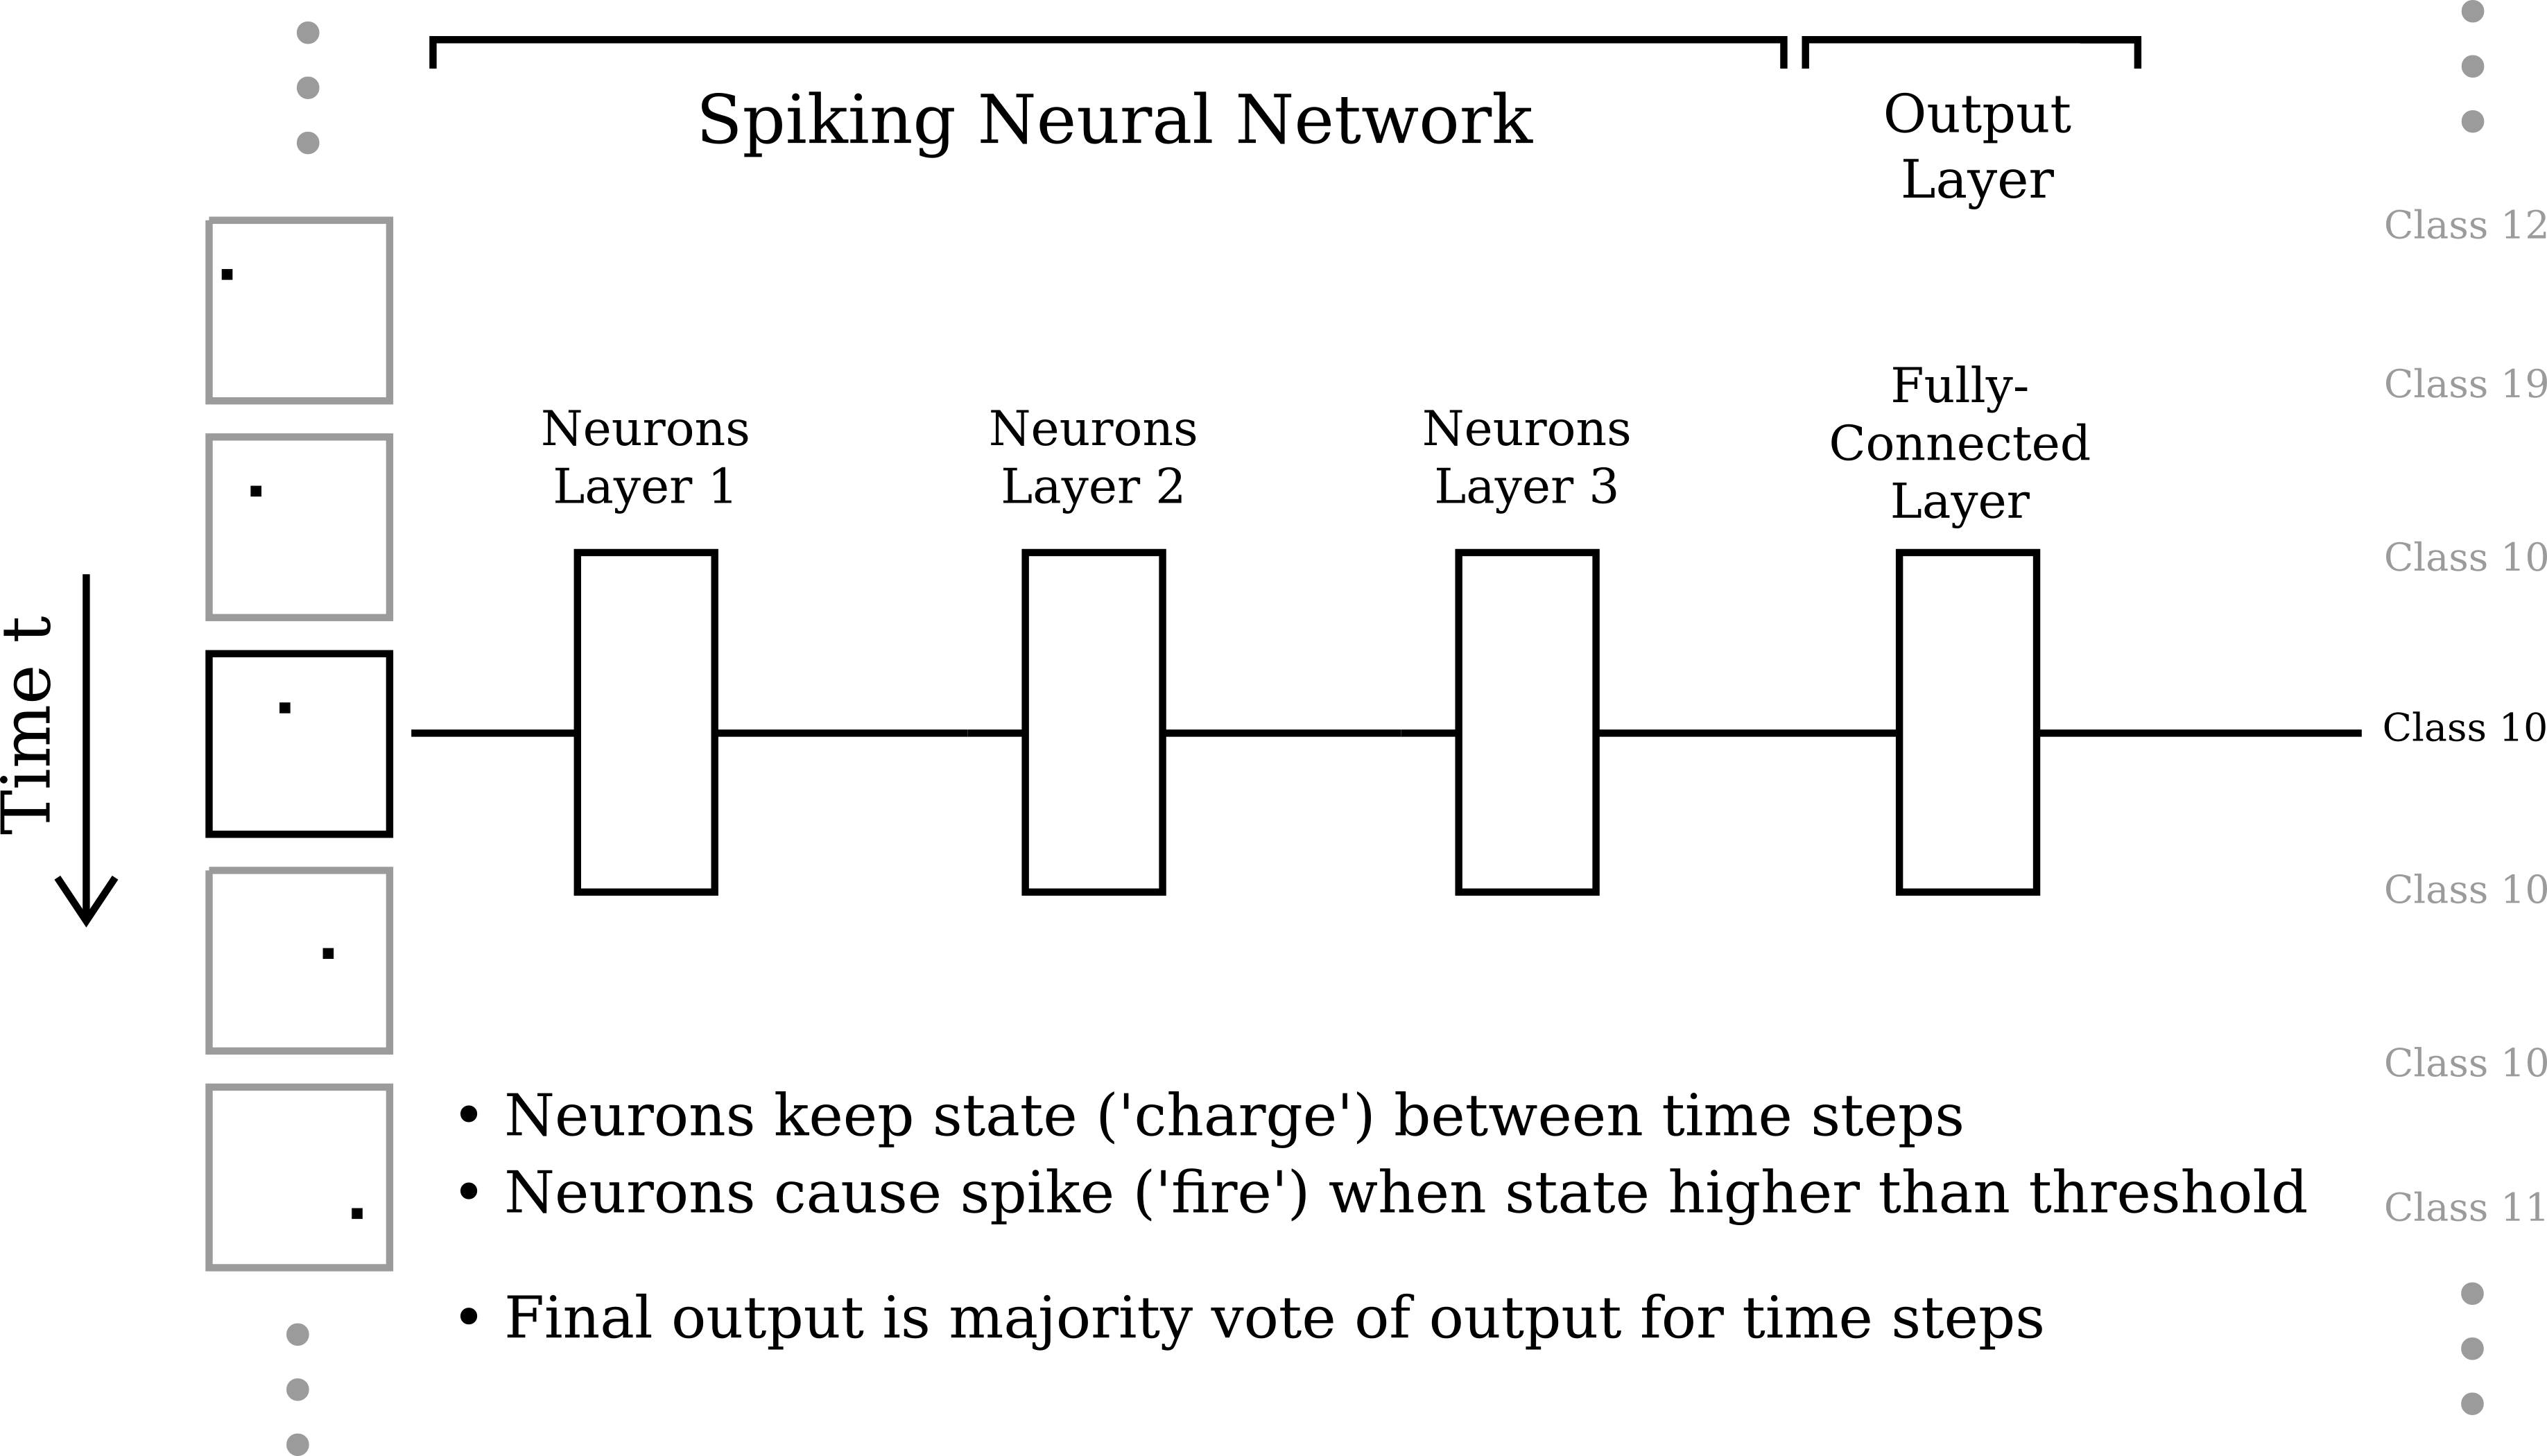
\includegraphics[width=0.8\textwidth]{network.png}
    \caption{High-level overview of network architecture.}
    \label{fig:network_arch}
\end{figure}

Although we spent a lot of time tuning hyperparameters for the SNN, we found it difficult to move past mid-50\% classification accuracies on the test set. For full 24-class classification, the peak per-SNR accuracy of our SNN model was 56\%.

\begin{figure}[H]
    \centering
    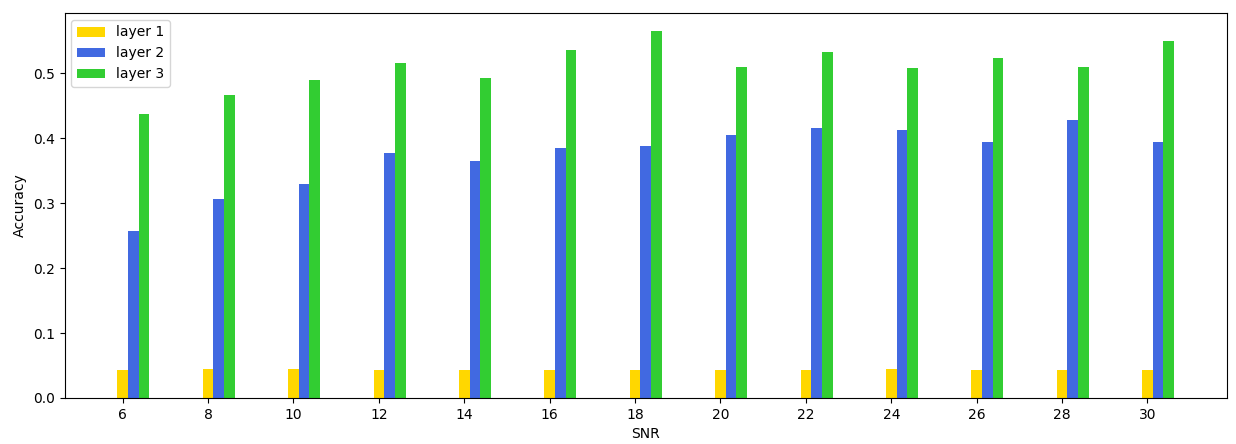
\includegraphics[width=\textwidth]{results_Jun12_06-28-21.png}
    \caption{Per-layer classification accuracies at different SNRs.}
    \label{fig:snr_results}
\end{figure}

\subsection{Adapting DCLL for Brevitas}

\label{sec:dcll_brevitas}

\subsubsection{Static Parameters}

To quantize the weights of the spiking neural network, we extended the \texttt{Conv2dDCLLlayer} class to a new class \texttt{QuantConv2dDCLLlayer}. This is similar to the way the \texttt{QuantConv2D} layer is built on top of \texttt{Conv2D} in the Brevitas library.

The \texttt{QuantConv2dDCLLlayer} uses the same weight tensor \texttt{self.weight} to store the precise floating point weights during the training process. However, the forward pass is modified so that the 
precise weights are quantized to a fixed integer bit width before being used to process the input. Similarly to the implementation of \texttt{QuantConv2D}, we used a \texttt{WeightQuantProxy} object for the purpose of quantizing the weights. Throughout the training process, Brevitas will maintain one single scale factor per layer which is applied to the integer values of the quantized weights and is rescaled automatically during the training process to allow the weights to make best use of the available bit width.

\subsubsection{Runtime Parameters}

In SNNs it is important to keep track of the internal neuron state (membrane potential) throughout time.
The next state value is calculated from a function of input, weights, and previous state. To quantize the state variables, it doesn't make sense to use dynamic scaling during the training process (as was used for weight quantization) since the state constantly changes during runtime and we need a permanent scale value for the device that the SNN is going to be run on.

To determine such a scale factor, the expected range has been measured experimentally by applying the test set on the network and storing maximum and minimum state value throughout computation. A \texttt{QuantIdentity} function is then used in Brevitas to fit integer variables of a certain bit width into an interval of real numbers (between 0 and the maximum value of the state determined experimentally, plus an added safety interval to allow the state higher values then the highest value measured in experiments). The Brevitas \texttt{QuantIdentity} function will, given the maximum value, automatically determine the scale factor applied to the raw integer values in order to get the state value adjusted to the desired range.

This is implemented as separate class \texttt{QuantContinuousConv2DState} which is a built on top of and as a replacement for \texttt{QuantContinuousConv2D}. While the latter class only supports weight quantization, the former can be used for both state and weight quantization.

\subsection{Evaluating Quantized SNN for RadioML}

We evaluated the quantized model on different bit widths to see how the reduced number precision would impact the overall model performance. Interestingly, the model is relatively tolerant to weight quantization. Even aggressive quantization of the model weights to 2-bit integers does not lead to a drop in accuracy of more than -5\%.

The internal neuron state is much more sensitive to lower precisions. Quantizing the state variables to 12-bit integers already causes the accuracy to be halved compared to the non-quantized  model.

\begin{figure}[H]
    \centering
    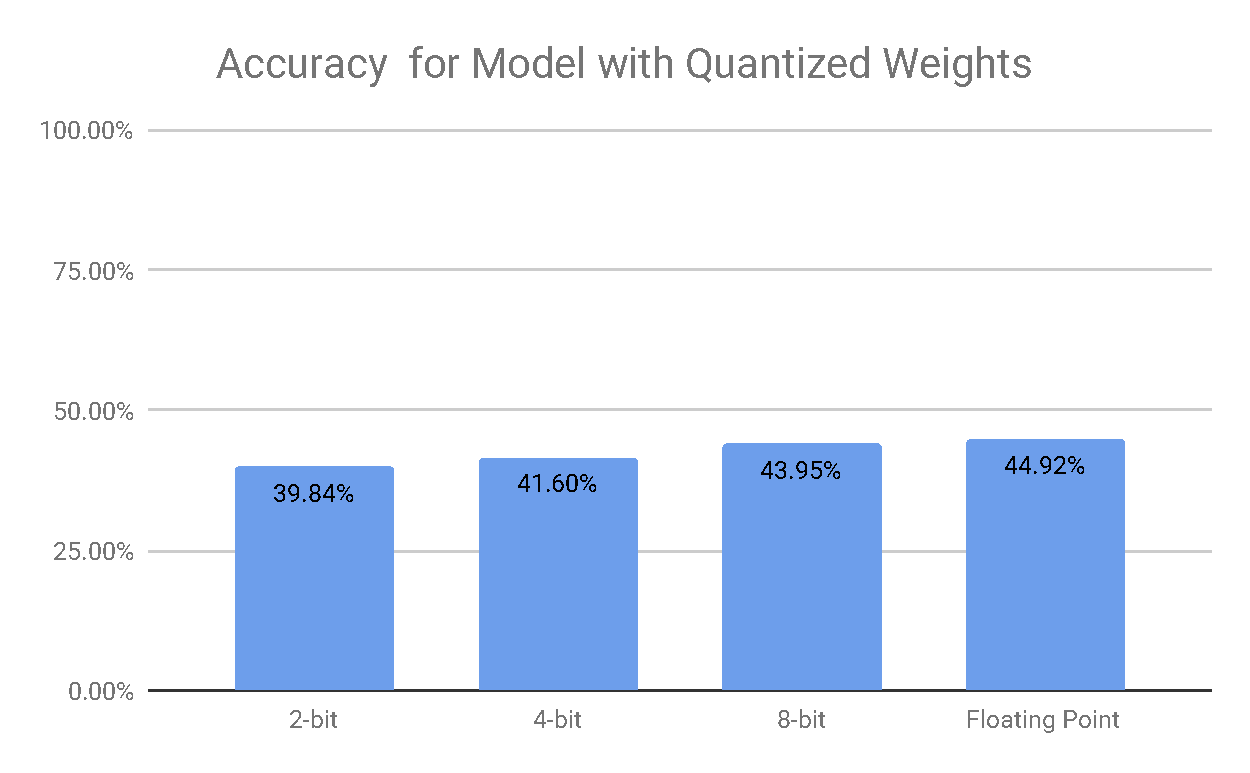
\includegraphics[width=0.5\textwidth]{quantized_weight.pdf}
    \caption{Model accuracy for quantized weights.}
    \label{fig:quantized_weights_result}
\end{figure}

\begin{figure}[H]
    \centering
    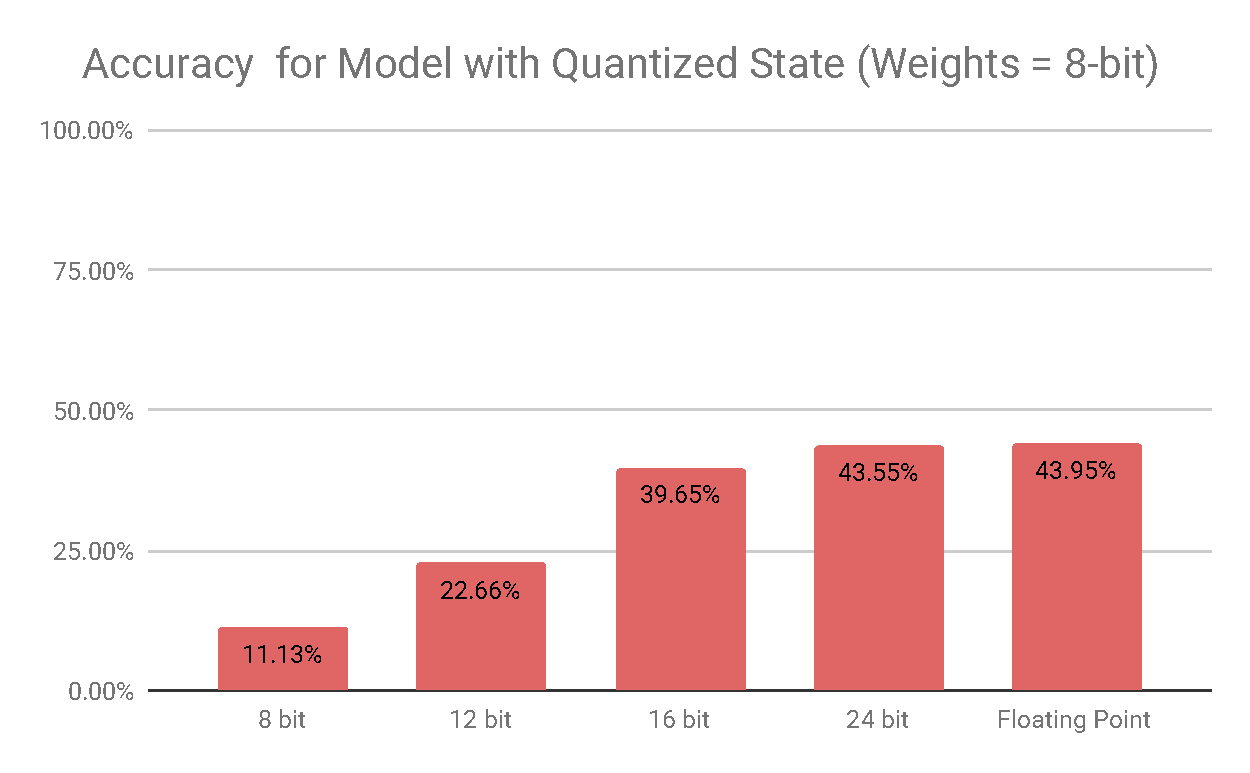
\includegraphics[width=0.5\textwidth]{quantized_state.pdf}
    \caption{Model accuracy for quantized state.}
    \label{fig:quantized_state_result}
\end{figure}
% Show the test results

\subsection{Proposed Quantized Architecture and Results}

Based on the evaluation results, we chose a weight quantization of 8-bit and a state quantization of 24-bit. This leads to a memory reduction for weights by 75\% for the neuron state of 25\% compared to a model using floating point parameters, while reducing the classification accuracy on the dataset by 1.37\%.

The following image is an illustration of a quantized DCLL layer. The network in total again consists of three convolutional DCLL layers followed by a fully-connected layer (non-spiking) which connects to the membrane potential of the neurons of the last layer.

\begin{figure}[H]
    \centering
    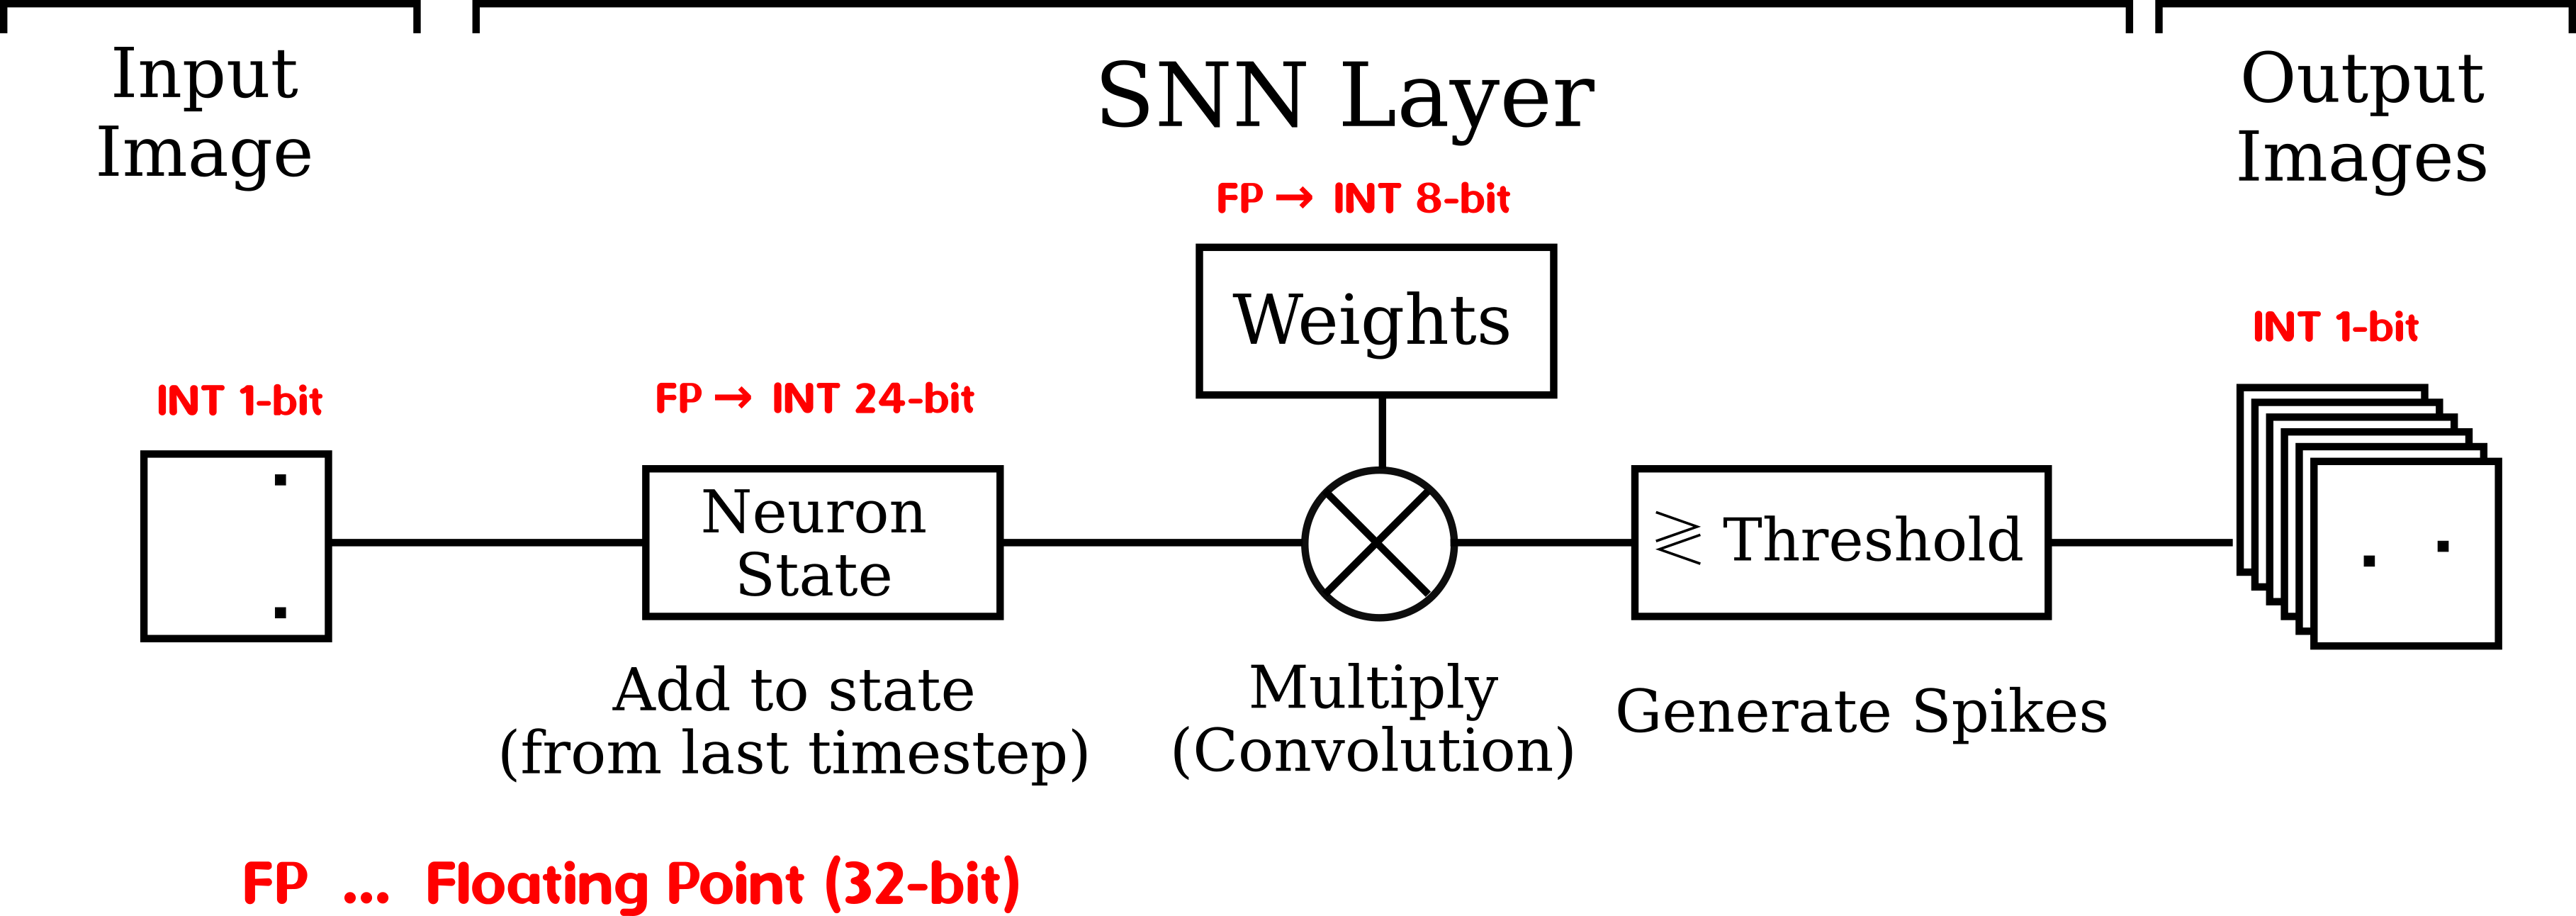
\includegraphics[width=0.8\textwidth]{quantization.png}
    \caption{Architecture of quantized layer.}
\end{figure}


\section{Conclusion}

In this project, we conducted, to our knowledge, the first foray into using spiking neural networks for automatic modulation classification on RadioML. We integrated DCLL SNNs, RadioML, and Brevitas into a multi-component system capable of classifying radio signals using quantized spiking neural networks.

Unfortunately, our results remained rather subpar in comparison to state-of-the-art traditional networks, despite all of our efforts to tune things for the better. We suspect that this may be due to the limitations of the training method that we are using for spiking networks, or the subpar regularization that we are applying (as the network does much better on the training set than it does on the test set).

Nevertheless, as spiking neural networks and event-based communication grow as a field of interest for the AI/ML community (for example, event-based cameras are gaining traction in computational photography, meaning visual domains may soon have a greater use for spiking-type networks), new training methods will be developed that may help close the gap between SNNs and residual networks on modulation classification. Furthermore, we consider it a promising sign that our network is able to achieve near-perfect accuracy on the training dataset, showing that it likely possesses the necessary representational capacity to solve the problem and simply needs to be regularized in some better and potentially SNN-specific way.

Finally, one (motivating) advantage that SNNs have over their traditional counterparts is efficiency; with the adoption of specialized and increasingly prevalent neuromorphic hardware, SNNs can be made to only process the ``events" and thus operate much more efficiently than most previous methods. Over time, as new methods drive the accuracy for SNN-based 24-modulation classification upward from our best result of 56\%, SNNs will likely become increasingly attractive as the accuracy gap lessens and the efficacy-efficiency tradeoff shifts in favor of SNNs on neuromorphic hardware.
\newpage
\section{Milestones}

In this section we include the original schedule for the project including the proposed milestones and address progress made throughout the project and how the milestones were completed.

Broadly, we were able to tackle every milestone, but we struggled to increase the performance of the SNN to above 60\% on our RadioML test set.

\label{sec:schedule}
\renewcommand{\arraystretch}{1.5}

\begin{table}[H]
\begin{tabularx}{\textwidth}{llm{9cm}l}
\toprule
\textbf{\textsf{Week}}    & \textbf{\textsf{Type}}            & \textbf{\textsf{Description}}                                                                             & \textbf{\textsf{}} \\
\midrule
4  & Milestone   & Train SNN (DCLL lib) with MNIST dataset                       & Simon          \\
        & Milestone   & Preprocess and load RadioML dataset for SNN                     & Owen           \\
\midrule
5  & Milestone   & Get familiar with Brevitas library                                                       & Simon          \\
        & Milestone   & Get familiar with the DCLL codebase                             & Owen           \\
\midrule
6  & Milestone & Extend Brevitas for usage with SNNs from dcll library & Simon          \\
        & Milestone & Adapt SNN for RadioML using DCLL PyTorch library                 & Owen           \\
\midrule
7  & Deliverable   & Hyperparameter tuning of SNN for RadioML                         & Simon          \\
        & Deliverable   & Hyperparameter tuning of SNN for RadioML                         & Owen           \\
\midrule
8  & Milestone   & Adapt RadioML SNN for quantization in Brevitas                                                                   & Simon          \\
        & Milestone   & Tuning of architecture parameters for RadioML SNN                                                                   & Owen           \\
\midrule
9  & Deliverable & Optimize quantized version of RadioML SNN                                               & Simon          \\
        & Deliverable & Optimize quantized version of RadioML SNN                                           & Owen           \\
\midrule
10 & Deliverable & Final report and video (focus: quantization)                                    & Simon          \\
        & Deliverable & Final report and video (focus: SNN implementation)                              & Owen    \\
\bottomrule
\end{tabularx}
\caption{Summary of milestone/deliverable schedule.}
\label{milestone_summary}
\end{table}

\section*{Week 4}

\textbf{\textsf{Simon}}:

\begin{tabularx}{\textwidth}{p{3.5cm} p{10cm}}
\underline{Description}: & Train SNN (DCLL lib) with MNIST dataset.\\

\underline{Completion Criteria}: & Have an SNN network that can be run on the MNIST dataset on the GPU cluster.\\
\underline{Completion}: &
\end{tabularx}
 \begin{itemize}
    \item{Configured job on GPU cluster to work with DCLL library}
    \begin{itemize}
        \item{Issue faced: Allocate RAM to allow training process to proceed properly without crashing while keeping utilization high} 
    \end{itemize}
    \item{Trained the default MNIST SNN on the cluster, peak accuracy: 99.02\%
    \begin{figure}[H]
        \centering
        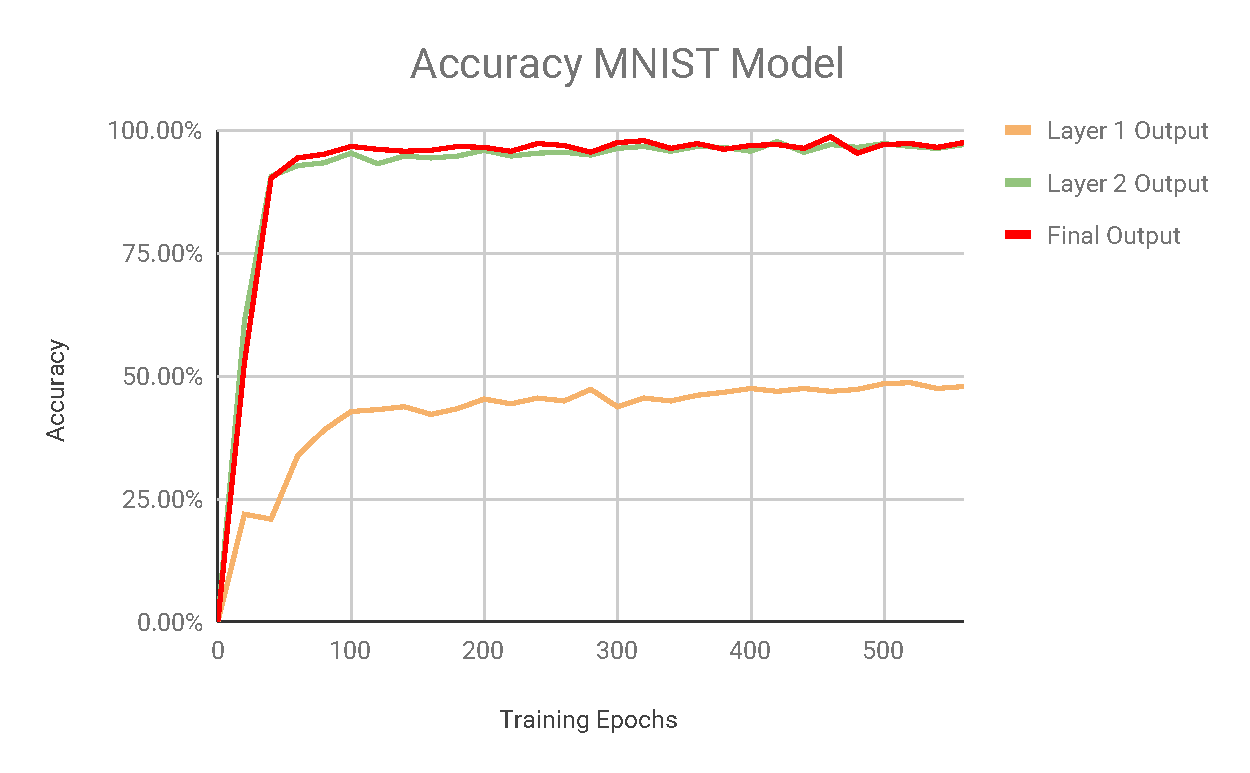
\includegraphics[width=0.5\textwidth]{mnist_original.pdf}
        \caption{Accuracy throughout training process for default MNIST model.}
    \end{figure}}
\end{itemize}

\textsf{\textbf{Owen}}:

\begin{tabularx}{\textwidth}{p{3.5cm} p{10cm}}
\underline{Description}: & Preprocess and load RadioML dataset for SNN.\\

\underline{Completion Criteria}: & Have the RadioML data on the GPU cluster in a form that can be fed to the SNN. \\
\underline{Completion}:
\end{tabularx}

See the code on GitHub (along with the file histories) which will show that a version of RadioML loading and preprocessing was implemented in Week 4, and a better version is implemented now.

Currently, we split the RadioML data into (per-class, per-SNR) HDF5 files, load the data from there, and convert the time-series data into spike trains by transforming the signal input at each time step into a spike at the nearest binned spatial location on the I/Q plane. The relevant files are \href{https://github.com/ohjay/snn-modulation-classification/blob/master/data/load_radio_ml.py}{{\tt data/load\_radio\_ml.py}} (note: the previous text is a link), which does the initial HDF5 loading, and \href{https://github.com/ohjay/snn-modulation-classification/blob/master/data/utils.py}{{\tt data/utils.py}}, which performs the conversion to spike trains.

\section*{Week 5}

\textsf{\textbf{Simon}}: 

\begin{tabularx}{\textwidth}{p{3.5cm} p{10cm}}
\underline{Description}: & Get familiar with Brevitas library.\\

\underline{Completion Criteria}: & Written report including a description of which functionality Brevitas offers, how the codebase of Brevitas is organized, how it is used for regular neural networks and outline on where extensions for spiking neural networks will have to be made.\\
\underline{Completion:} &
\end{tabularx}

Refer to the description of Brevitas in section \ref{sec:brevitas}.

Important parts of the Brevitas code for this project are located in the following directories:
\begin{itemize}[noitemsep]
\item{\textbf{\textsf{nn:}} Defines higher level classes like convolutional and linear layers, activation function, batch normalisations with quantization support}
\item{\textbf{\textsf{proxy:}} Useful quite high-level structures for quantization e.g. to track weights and perform scaled quantization}
\item{\textbf{\textsf{core:}} Contains the low-level part of Brevitas defining a TensorQuant structure and IntQuant classes that
can e.g. quantize floating point values into the correct integer range given certain bit settings and a scale factor}
\end{itemize}

For the weight quantization, we will look at the implementation for the already provided \texttt{QuantConv2D}, a regular convolutional layer that builds upon \texttt{Conv2D} and takes the precise weights of the \texttt{Conv2D} part and quantizes them
during every forward pass. The implementation for the DCLL convolutional layer will work in similar fashion using
the \texttt{WeightQuantProxy} object.

\textsf{\textbf{Owen}}:

\begin{tabularx}{\textwidth}{p{3.5cm} p{10cm}}
\underline{Description}: & Get familiar with the DCLL codebase, determine which parts of the code will need to be changed in order to create a VGG-like SNN architecture using DCLL modules.\\

\underline{Completion Criteria}: & Written report which includes a high-level overview of the different parts of the code and a description of which specific files and functions will need to be changed or utilized in order to define a VGG-like architecture for use with RadioML.\\
\underline{Completion}: &
\end{tabularx}

Following is a written report, which could be expanded to a separate page upon request. After the refactor/cleanup, the code is split into four different folders: {\tt data}, {\tt dcll}, {\tt networks}, and {\tt scripts}. {\tt data} includes files that relate to the loading of specific datasets (currently the supported options are MNIST and RadioML) and preprocessing them -- converting them to spike trains, for example. {\tt dcll} includes files (largely unedited from those of the original authors) which implement the Deep Continuous Local Learning layers and define auxiliary experimental utilities. {\tt networks} includes a Python file which implements general architecture-building, and YAML files that specify, in a readable format, the architectures we use for our specific use cases (MNIST and RadioML classification). {\tt scripts} contains runnable training and testing scripts for MNIST and RadioML. Finally, in the root directory, there is the {\tt train.py} file which serves as an entry point for training. It sets things up according to command-line arguments and then runs a training/evaluation loop.

In order to define a VGG-like architecture for use with RadioML, we will need to change the YAML network specification in {\tt networks/radio\_ml\_conv.yaml}. And that should be it, since the code has been refactored to support generalized YAML-based network building. For hyperparameter tuning, the hope is that we will mainly just need to modify the command-line arguments in the launch scripts.


\section*{Week 6}


\textsf{\textbf{Simon}}:

\begin{tabularx}{\textwidth}{p{3.5cm} p{10cm}}
\underline{Description}: & Extend Brevitas for usage with spiking neural networks from dcll library.\\

\underline{Completion Criteria}: & Have a trained quantized version of the MNIST network for different bit sizes (16-, 8- and 4-bit) and report on accuracy achieved.\\
\underline{Completion}:
\end{tabularx}

The changes made to combine DCLL library code with the Brevitas framework is described in section \ref{sec:dcll_brevitas} of this report.

The weight quantization for the MNIST model achieved the following results:
\begin{figure}[H]
    \centering
    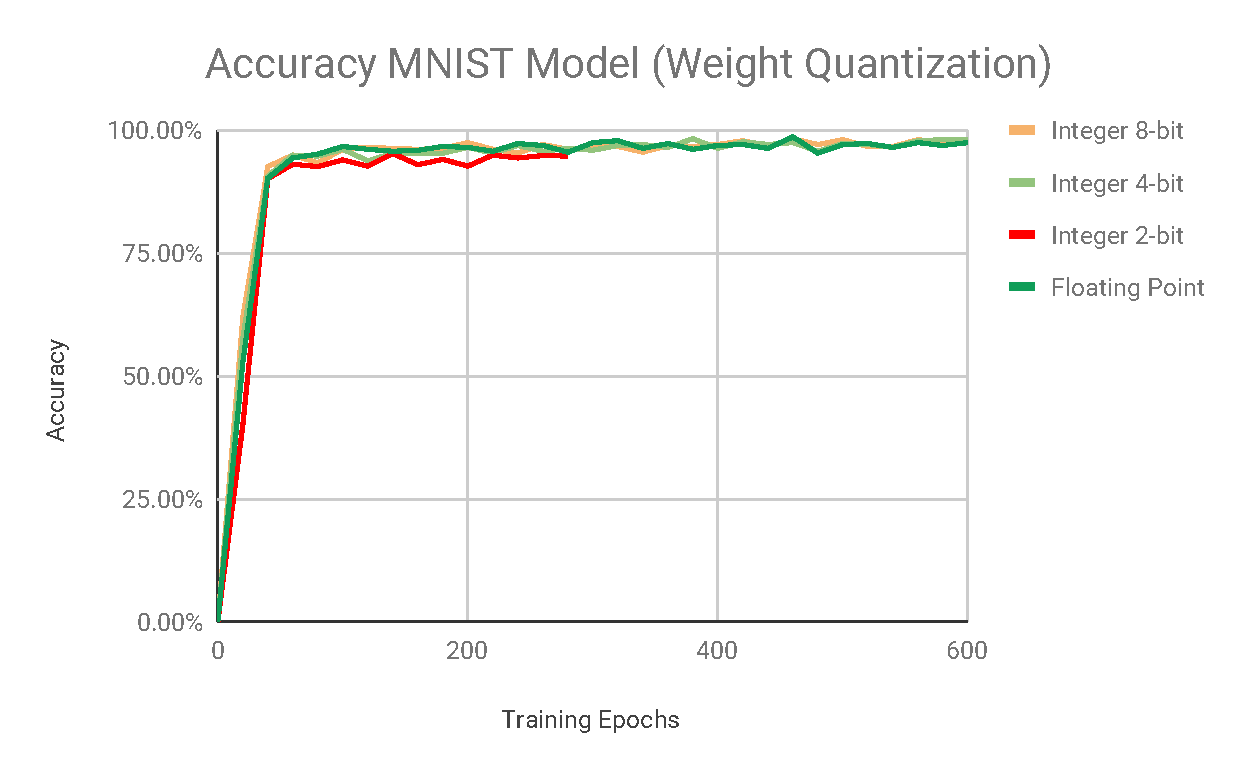
\includegraphics[width=0.5\textwidth]{mnist_quantization.pdf}
    \caption{Accuracy for MNIST SNN with quantized weights.}
\end{figure}

A summary of the results achieved using runtime quantization is shown below:
\begin{figure}[H]
    \centering
    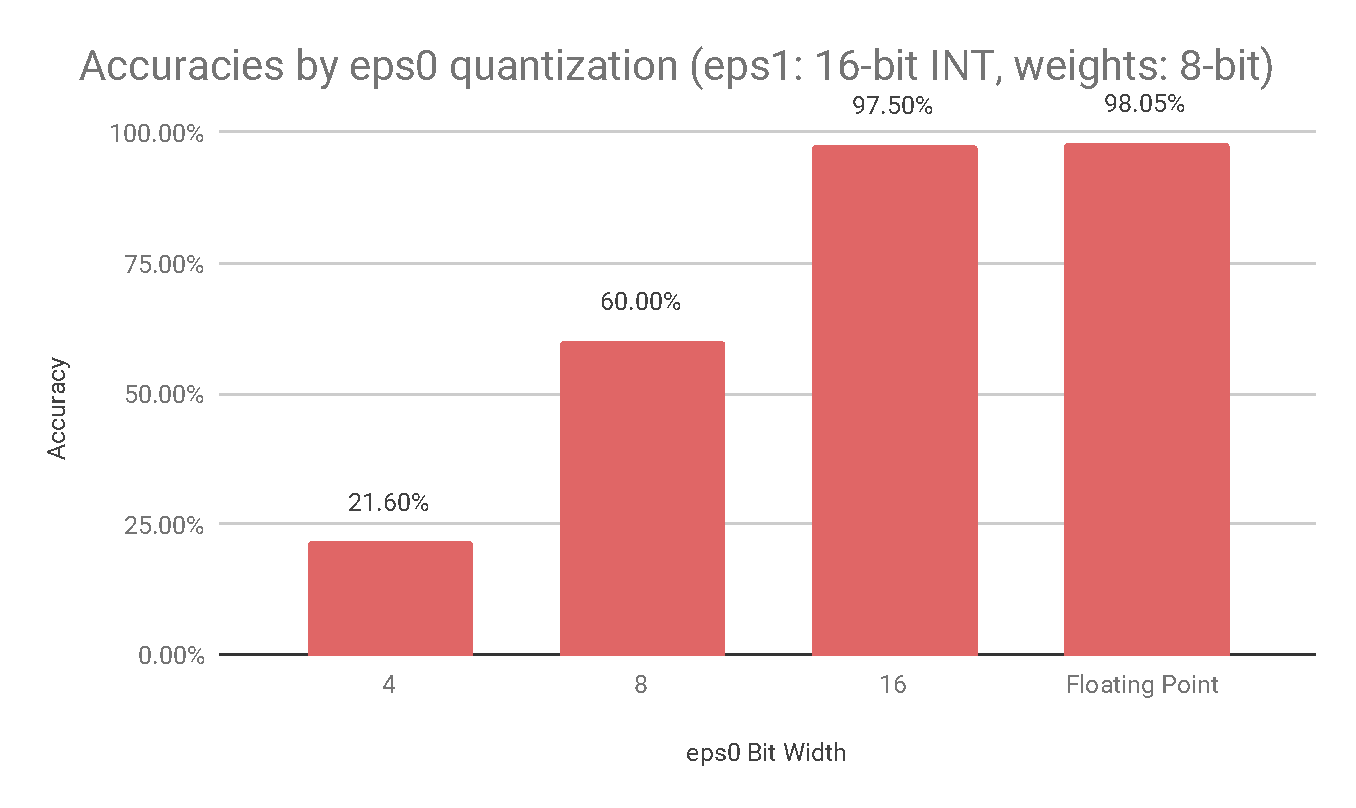
\includegraphics[width=0.4\textwidth]{eps0.pdf}~
    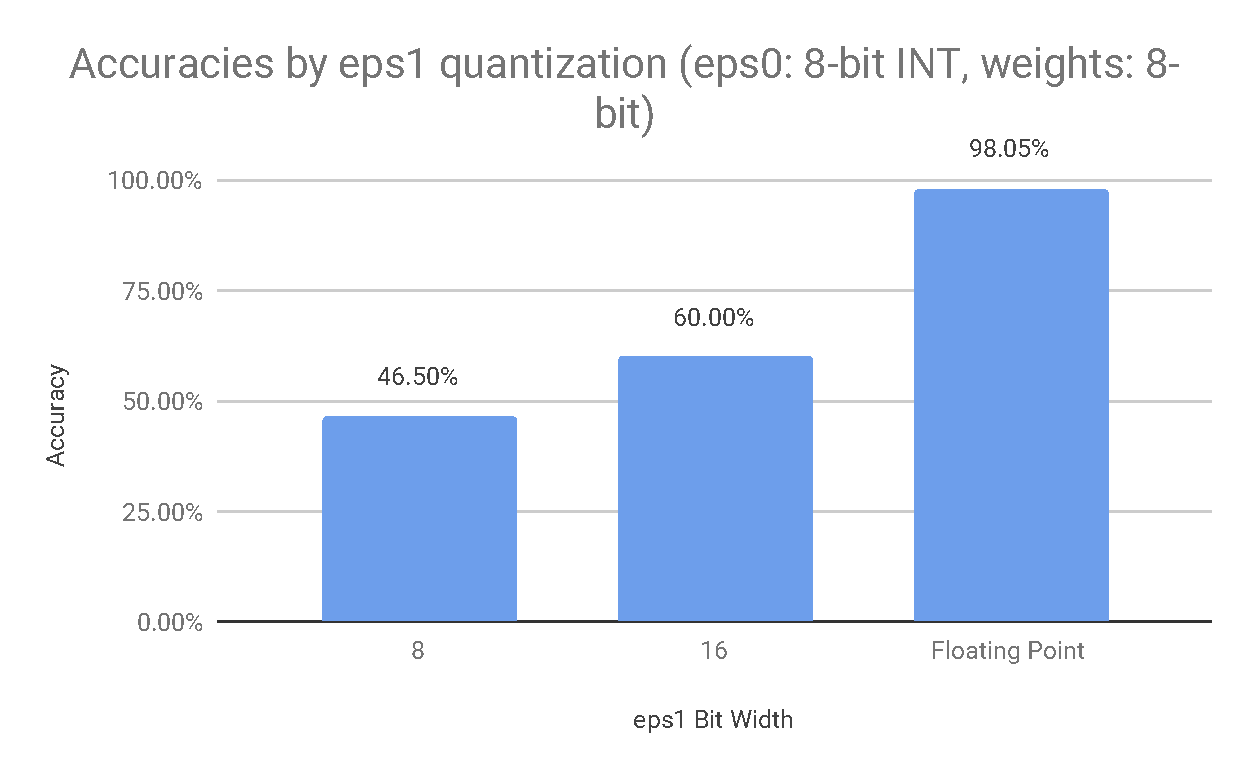
\includegraphics[width=0.4\textwidth]{eps1.pdf}
    \caption{Accuracy for different runtime quantization.}
\end{figure}

\textsf{\textbf{Owen}}:

\begin{tabularx}{\textwidth}{p{3.5cm} p{10cm}}
\underline{Description}: & Adapt SNN for RadioML using DCLL PyTorch library.\\

\underline{Completion Criteria}: & Have a first SNN modeled after VGG that can be trained on RadioML data (ignoring actual performance at this point). \\
\underline{Completion}: & By checking the history of \href{https://github.com/ohjay/snn-modulation-classification/blob/master/networks/radio_ml_conv.yaml}{\tt networks/radio\_ml\_conv.yaml} (the previous text is a link), you can see the specifications for the VGG-inspired networks that we set up. Furthermore, you can browse the different states of the codebase over the last few weeks, where we were able to train an SNN on RadioML data in almost all of them (pretty much every commit after week 4 should support SNN RadioML training -- just run {\tt scripts/train\_radio\_ml.sh} at any point in the history where the script exists).
\end{tabularx}

\begin{figure}[H]
\centering
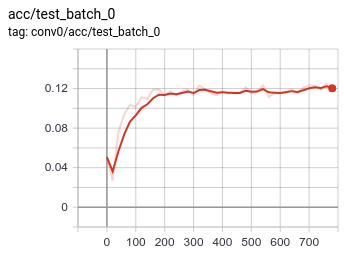
\includegraphics[width=0.3\columnwidth]{rml_snn_acc3.png}~
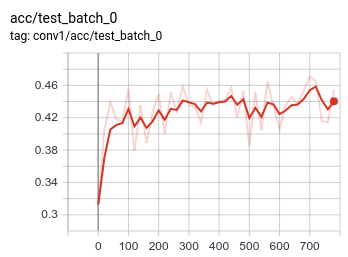
\includegraphics[width=0.3\columnwidth]{rml_snn_acc2.png}~
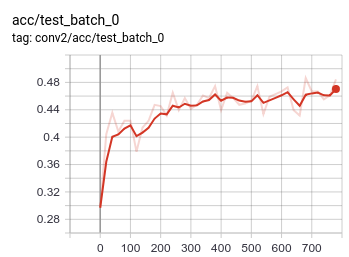
\includegraphics[width=0.3\columnwidth]{rml_snn_acc1.png}
\caption{An example of the training process on RadioML for each of three convolutional DECOLLE SNN layers. The plots depict mean validation accuracy over time.}
\end{figure}

\section*{Week 7 - Deliverable}

\textsf{\textbf{Owen \& Simon}}:

\begin{tabularx}{\textwidth}{p{3.5cm} p{10cm}}
\underline{Description}: & Hyperparameter tuning of SNN for RadioML\\

& Explore different versions for hyperparameters focusing on learning rate, learning rate decay schedule, optimizers, momentum, batch size, etc. to optimize achieved accuracy of the network.\\

\underline{Completion Criteria}: & Classify RadioML data by modulation with at least, say, 60\% accuracy on the test set (which corresponds to the worst performance reported in the previous work).\\

\underline{Deliver}: & Report on architecture, implementation and hyperparameters for the model and discuss resulting accuracy.\\
\underline{Completion:}& For results of the optimization process, refer to ``Tuning of SNN for RadioML network" section of the report.
\end{tabularx}

\section*{Week 8}

\textsf{\textbf{Simon}}:

\begin{tabularx}{\textwidth}{p{3.5cm} p{10cm}}
\underline{Description}: & Adapt RadioML SNN for quantization in Brevitas.\\

\underline{Completion Criteria}: & Have a trained quantized version of RadioML SNN in Brevitas (without focusing on accuracy at this point).\\
\underline{Completion}: &
\end{tabularx}

For this milestone, the SNN for RadioML from week 7 was adjusted to work with classes \texttt{QuantConvNetwork}, \texttt{QuantConv2dDCLLlayer}. Training of quantized weights worked without any further problems. For the state quantization, the accuracy initially dropped significantly. This was due to the maximum state value being poorly calibrated for the new type of data. After determining the new maximum value and readjusting the quantized state variable, the drop in accuracy was comparable to the experiments run on MNIST data in week 6.
\newpage
\textsf{\textbf{Owen}}:

\begin{tabularx}{\textwidth}{p{3.5cm} p{10cm}}
\underline{Description}: & Tuning of architecture parameters for RadioML SNN\\

& Hyperparameter tuning can be a very time-consuming and tedious process. Therefore, we schedule this week to continue
experimentation, focusing on modifications and optimizations of the model architecture.\\

\underline{Completion Criteria}: & Have optimized RadioML SNN with highest achieved accuracy, update report with results.\\
\underline{Completion}: &
\end{tabularx}

We did continue to tune hyperparameters and re-train networks throughout these weeks (for more details, see ``Tuning of SNN for RadioML network" in the Technical Material section of this report). However, despite our best efforts, the gains in accuracy were marginal, going from around 49\% to 54\%.

\section*{Week 9 - Deliverable}

\textsf{\textbf{Owen \& Simon}}:

\begin{tabularx}{\textwidth}{p{3.5cm} p{10cm}}
\underline{Description}: & Optimize quantized version of RadioML SNN.\\

& Experiment with the Brevitas model for RadioML to reduce model size while maintaining high accuracy.\\

\underline{Completion Criteria}: & Have optimized quantized RadioML SNN with highest achieved accuracy.\\

\underline{Deliver}: &  Report on architecture, implementation and hyperparameters for quantized RadioML SNN.\\
\underline{Completion}: &
\end{tabularx}

The network was trained and evaluated using different bit widths for weights and neuron state to optimize the performance and find a trade-off between accuracy and resource consumption of the network. 

\begin{figure}[!h]
\centering
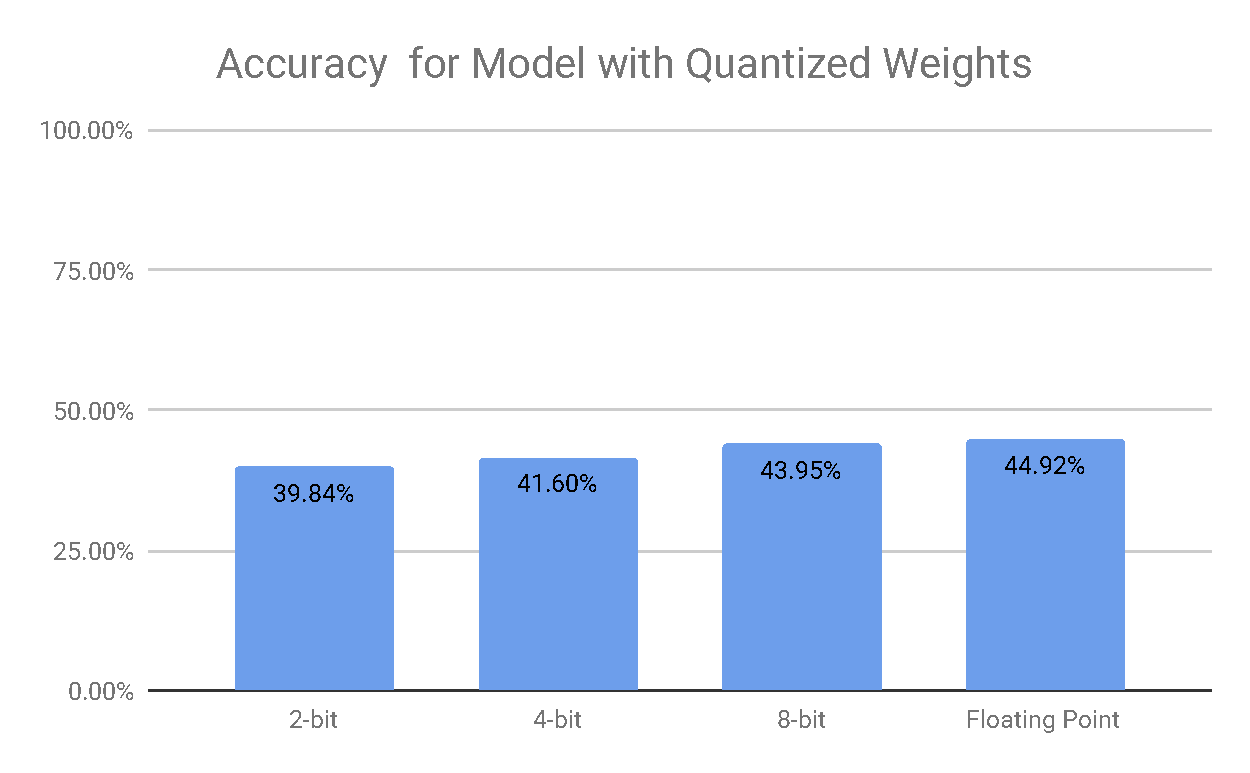
\includegraphics[width=0.5\columnwidth]{quantized_weight.pdf}~
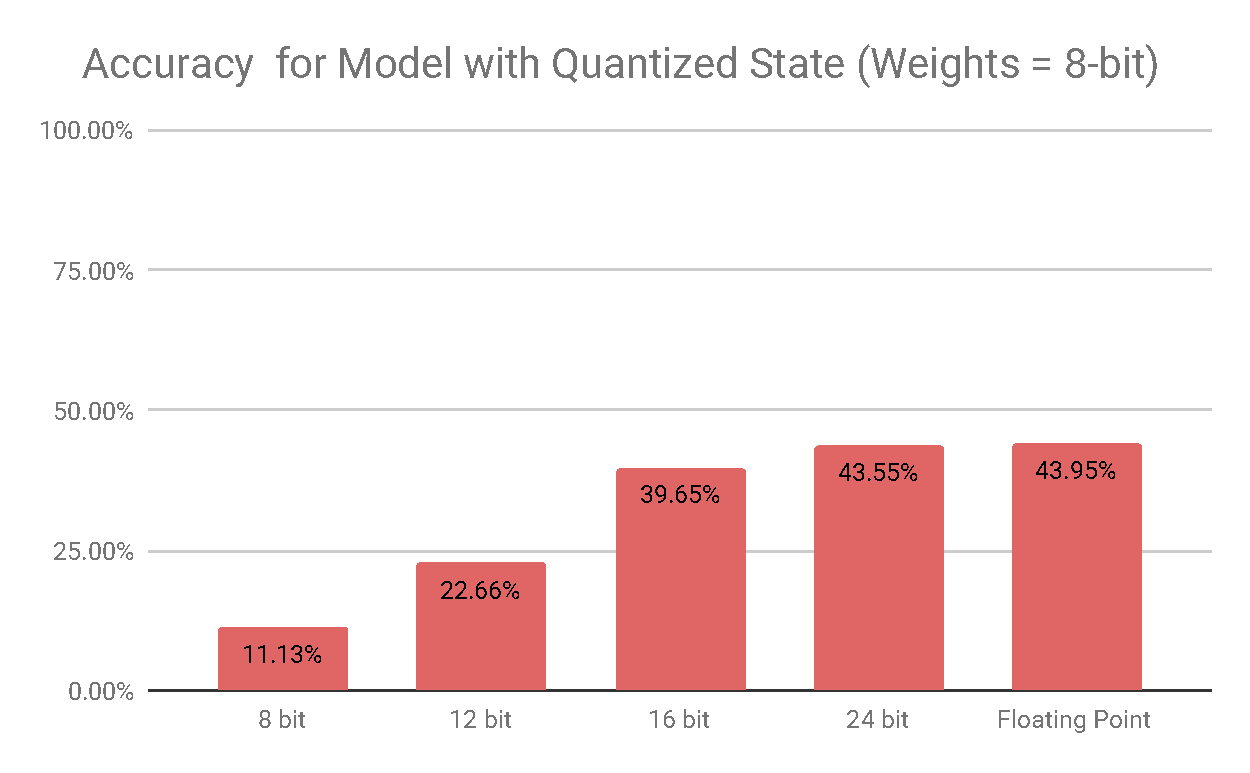
\includegraphics[width=0.5\columnwidth]{quantized_state.pdf}
\caption{Accuracy for different quantization bit widths.}
\end{figure}

For the proposed network we chose a weight quantization of 8-bit and a state quantization of 24-bit. This leads to a memory reduction for weights by 75\% for the neuron state of 25\% compared to a model using floating point parameters while reducing the classification accuracy on the dataset by 1.37\%.

\section*{Week 10 - Deliverable}

\textbf{\textsf{Owen \& Simon}}:

\begin{tabularx}{\textwidth}{p{3.5cm} p{10cm}}
\underline{Description}: & Final report and video\\

\underline{Completion Criteria}: & Submit final report and video addressing project progress, challenges, solutions and results.\\
\underline{Completion}: &
Final report submitted and video introduction to the project uploaded to Youtube. Video and documentation can be found on the project webpage \url{https://iot-lif.github.io/}.
\end{tabularx}


\nocite{*}
\bibliographystyle{unsrt}
\bibliography{bib}

\end{document}
